\begin{center}
  \Large
  \textbf{BIOGRAFI PENULIS}
\end{center}

\addcontentsline{toc}{chapter}{BIOGRAFI PENULIS}

\vspace{2ex}

\begin{wrapfigure}{L}{0.3\textwidth}
  \centering
  \vspace{-3ex}
  % Ubah file gambar berikut dengan file foto dari mahasiswa
  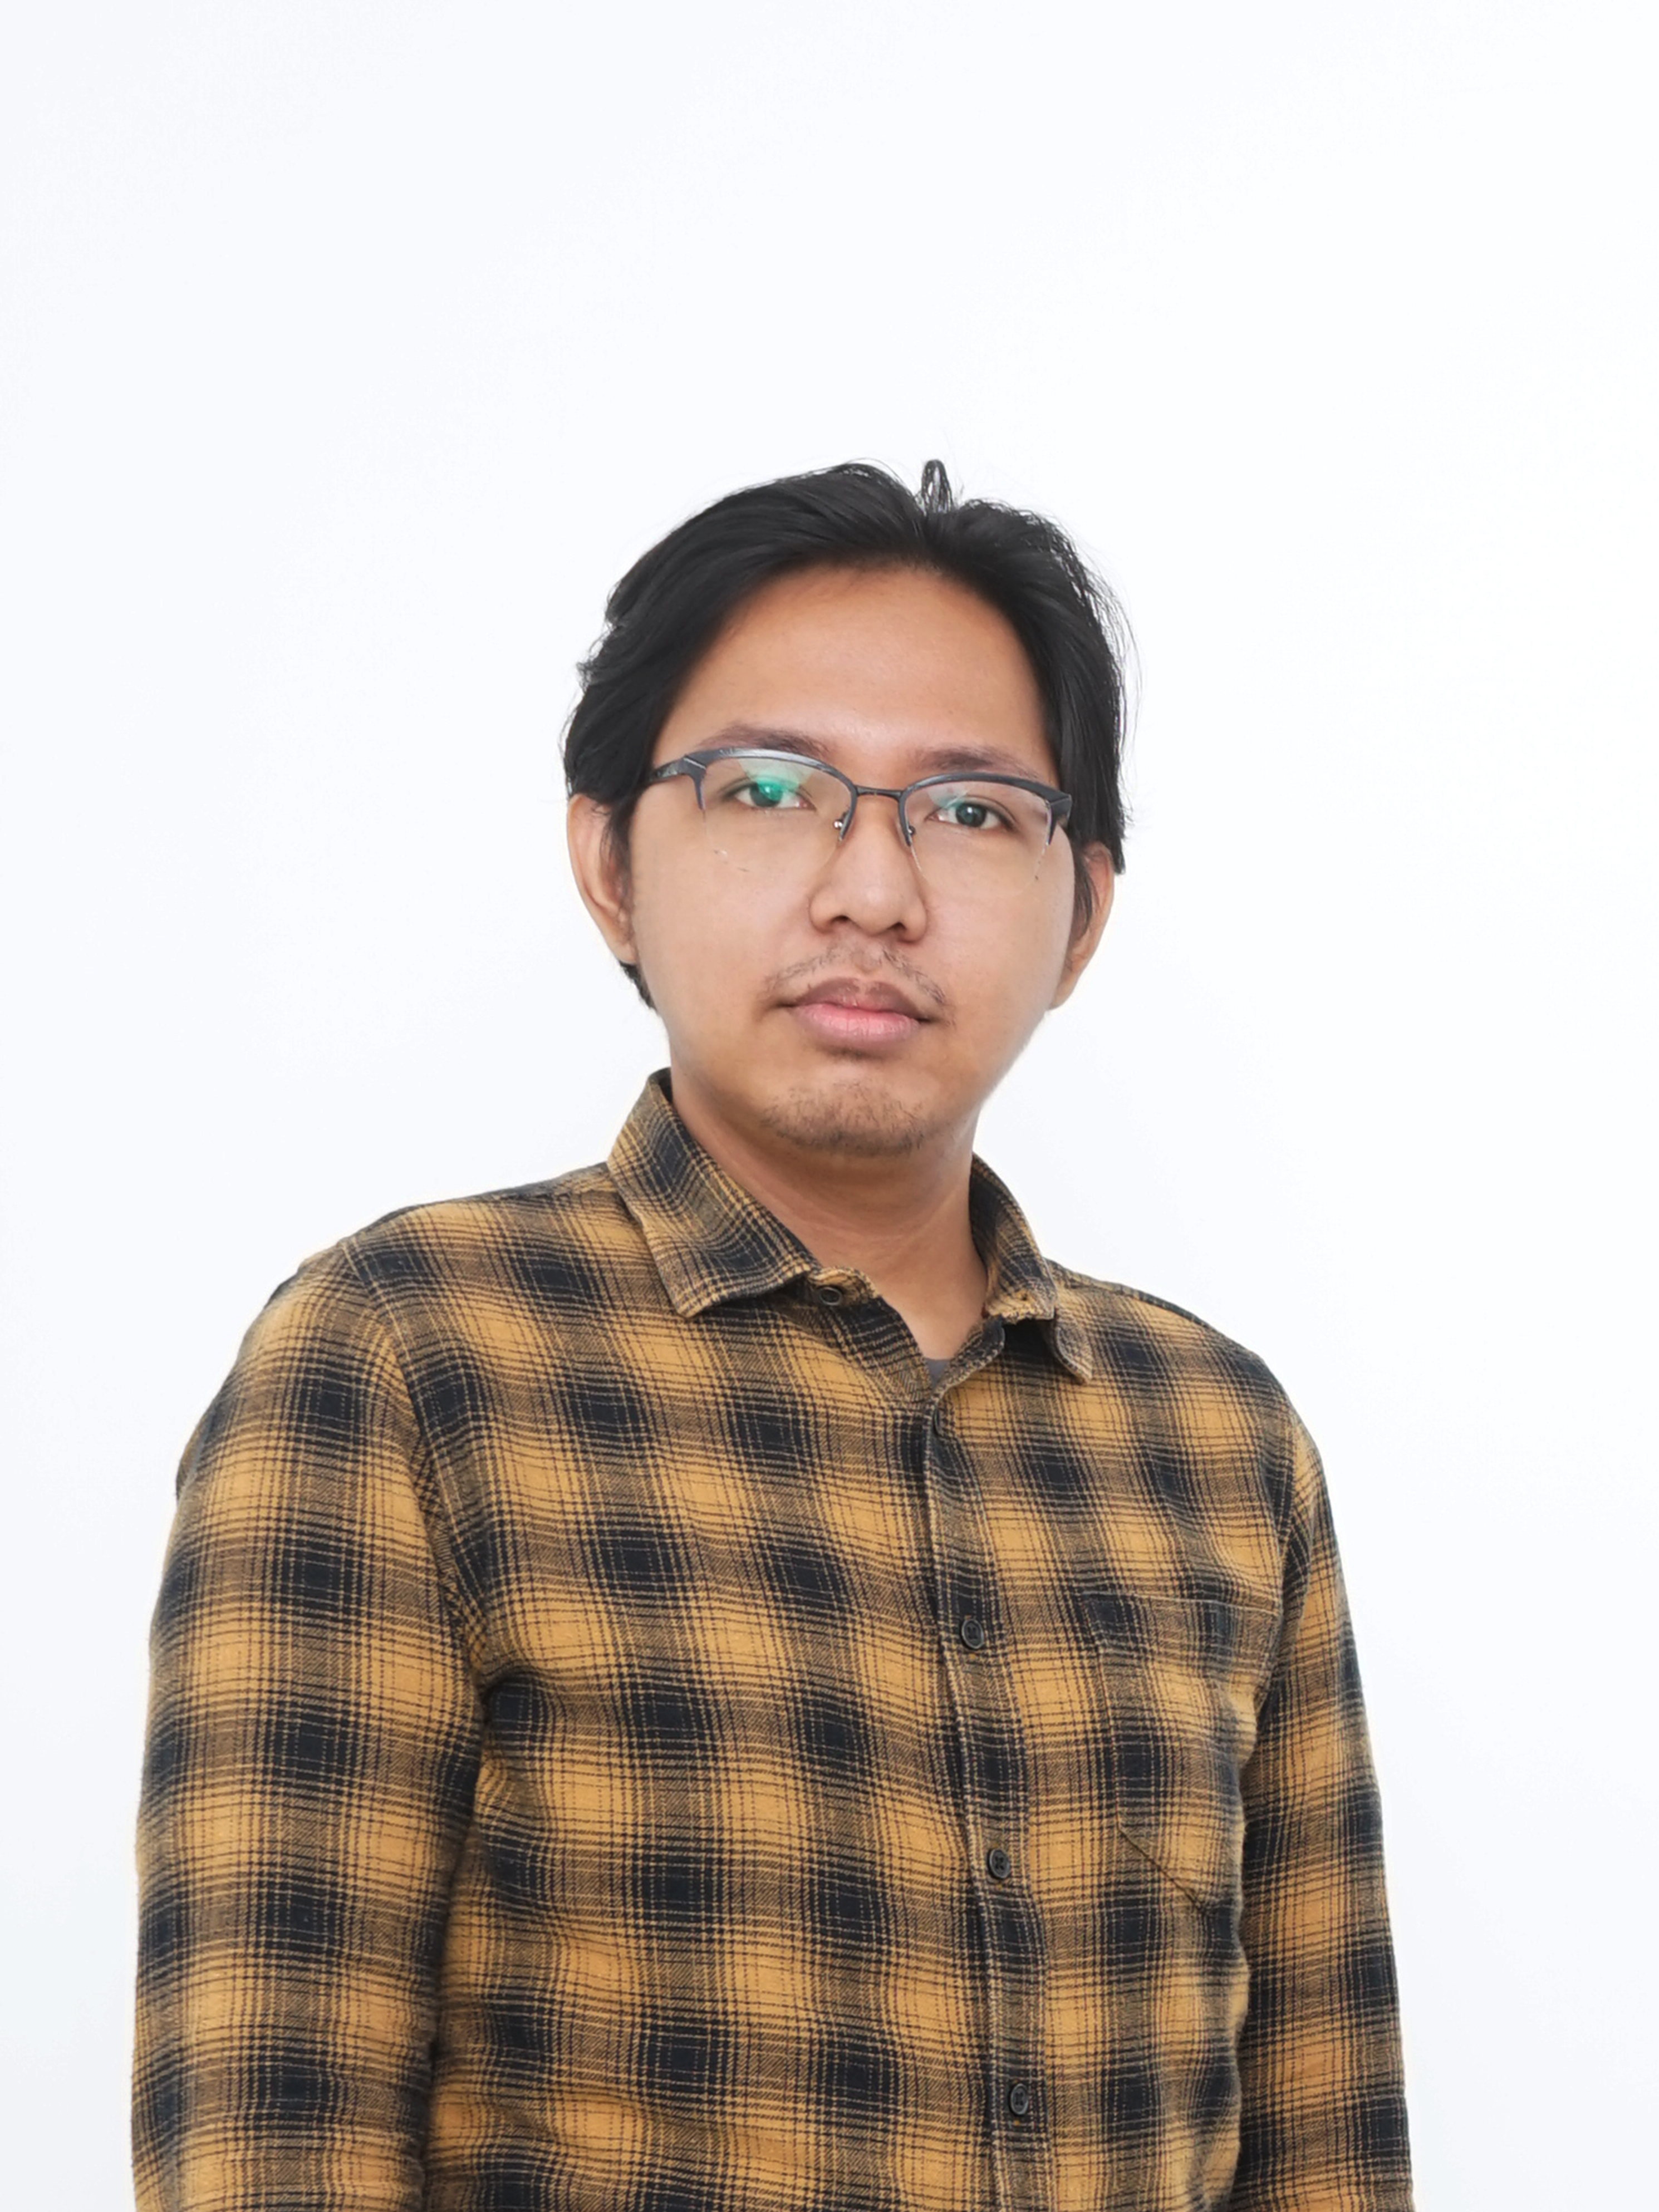
\includegraphics[width=0.3\textwidth]{gambar/dimas.jpg}
  \vspace{-4ex}
\end{wrapfigure}

% Ubah kalimat berikut dengan biografi dari mahasiswa
Dimas Nazli Bahaduri, lahir pada 20 Mei 2000 adalah anak terakhir dari tiga bersaudara dari Ibu Kusmiati dan Alm. Abdul Rauf. Dimas Nazli Bahaduri adalah anak yang pendiam sejak lahir dan suka melakukan perincian bahkan merusak berbagai benda-benda di sekitarnya hanya untuk keingintahuannya. Merasa tertarik dengan dunia yang imajiner, dia memiliki hobi menggambar dan melebar ke berbagai bentuk seni gerak, suara, hingga citra. Selain memiliki hobi yang bersinggungan dengan dunia seni, dia juga suka untuk mempertanyakan  sekitar berkat ketidak-sengajaannya membaca Kongzi. Salah satu ajaran yang digaungkan kembali oleh Kongzi adalah sadar untuk menjadi siapa dan seutuhnya menjadi sesuai kemampuannya. Maka dari itu Dimas bercita cita mempunyai studio Animasi untuk anak anak bertalenta dan menimba ilmu sebanyak dan sekomprehensif mungkin. Semua itu berangkat dari momen abangnya yang berkuliah selama 3 tahun dan lulus pada tahun 2006 dari sekolah kedinasan. 
\\Rejeki pun menempatkan Dimas di Insitut Teknologi Sepuluh Nopember di jurusan Teknik Komputer.Mengenyam bangku perguruan tinggi membuka pandangan baru seorang Dimas dan berkontribusi mengasah potensi, kemampuan, dan keinginannya. Melalui berbagai kegiatan organisasi hingga UKM telah ia coba. Ditambah dengan antusiasme dia kepada komputer dan seni digital membuat dia semakin yakin untuk berkuliah di Teknik Komputer ITS. Setelah menempuh kuliah 3.5 tahun lebih di Teknik Komputer menambah pengetahuan dan arti terjatuh, terbangun, senang, susah, kebingungan, hingga bersyukur. Tentu dia merasa beruntung dan bersyukur karena bertemu dosen, tenaga pendidik, staff, teman, kakak tingkat, hingga warga sekitar. Meskipun suatu saat dia tidak akan selamanya di Teknik Komputer,dia merasakan dampaknya dan kebajikan yang dia dapatkan akan dituang di kehidupan selanjutnya. 

